%%% -*-LaTeX-*-

\chapter{Migration Protocol}
We have seen that the current generation of NICs are capable of transferring Gigabytes of 
data per second in latencies of the order of a few microseconds and we have reasons to believe 
that the next generation of networking hardware will have the ability to process 
hundreds of millions of messages per second at bandwidth of the order of tens of Gigabytes per 
second and sub microsecond latencies\cite{cx6}.
We saw from the previous chapters how the nuanced performance characteristics of 
a modern NIC will influence overall transmit performance and server resource utilisation 
for large data transfers such as responses to range scans. Yet another pressing 
concern for a modern In-memory database operating at scale is quick reconfiguration. 
Since DRAM is the most expensive resource in a modern cluster, efficient rebalancing 
involves fast reconfiguration that is frugal on resources and keeps the impact on their 
SLAs minimal.
Informed with our lessons about the NIC, it is reasonable to assume that protocols for reconfiguration 
today can benefit from these optimisations and armed with these, they might come 
closer to what the hardware is capable of doing today.

In this Chapter, we discuss the state of the art migration protocols and their 
performance, does an analysis of the existing migration protocol in RAMCloud, 
and armed with the lessons learned by profiling a modern NIC, we make concrete 
suggestions on how a new protocol might be well poised to take advantage of the 
new hardware.


\section{State of the art}

\section{Migration in RAMCloud}

\section{Locality in RAMCloud}

\begin{figure}[t]
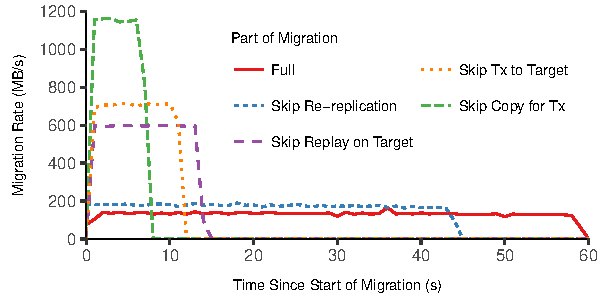
\includegraphics{fig-bottlenecks.pdf}
\caption{Bottleneck plot}
\label{fig:deltas}
\end{figure}

\begin{figure}[H]
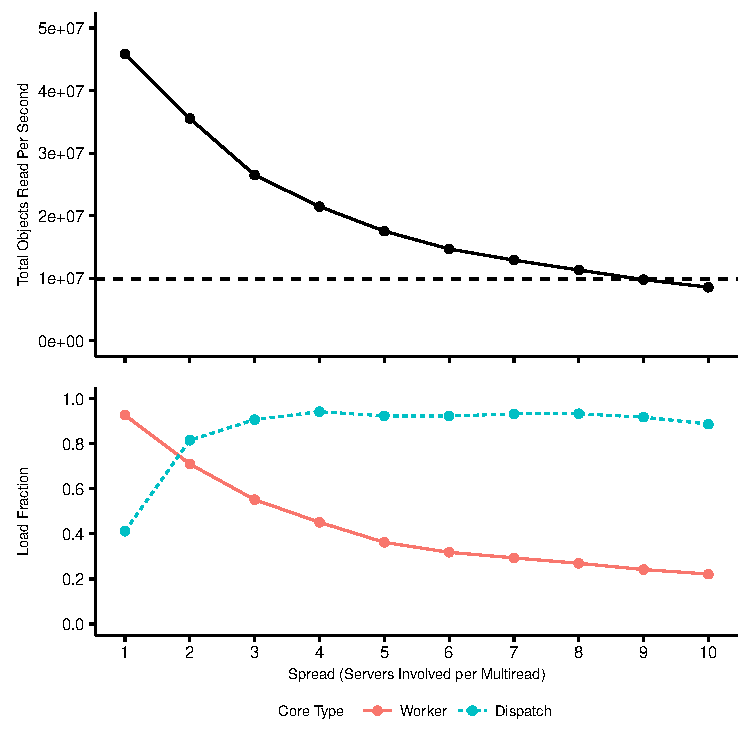
\includegraphics{fig-colocation.pdf}
\caption{Colocation plot}
\label{fig:colocation}
\end{figure}
